\begin{problem}{/images/problems/pic.jpg}{Finding the Area (II)}
In the figure below, a circle with a radius of 2 is tangent to the center of the side of a half-circle with a radius of 3, and a square is surrounded by their intersection.\\[0.2cm]

What is the area of the green part?

\begin{center}
	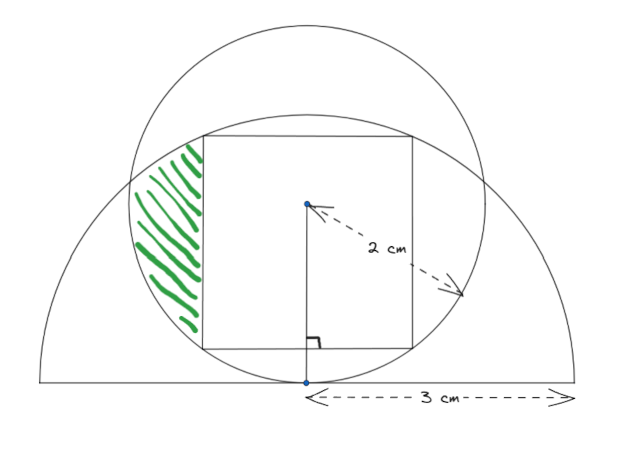
\includegraphics[width=9cm]{/images/problems/25_area.png}
\end{center}

\end{problem}
\begin{solution}
The answer to the question is $1.349$.\\[0.2cm]
 \noindent In the first step, we find the length of the sides of the square, which is approximately 2.36822, and the x coordinate of the left side of the square which is $x_4 \simeq -1.18411$. In the second step, we find the area of the intersection of the red circle and the green semicircle. We know that $y_3 = 2.25$. Now, putting it in the semicircle formula, we get: $$ x_3^2+y_3^2 = 3^2 \quad \implies \quad x_3 \simeq -1.98431 $$ Now, if we look closely at the target area, it can be divided into 3 parts: 
 \begin{itemize}
 \item \textbf{green section} which is located between the green semicircle and the line $x=2$. 
 \item \textbf{red section} which is located between the line $x=2$ and the lower half of the red circle. 
 \item \textbf{blue section} which is located between the upper half of the red circle and the line $x=2$. 
 \end{itemize}
\begin{center}
	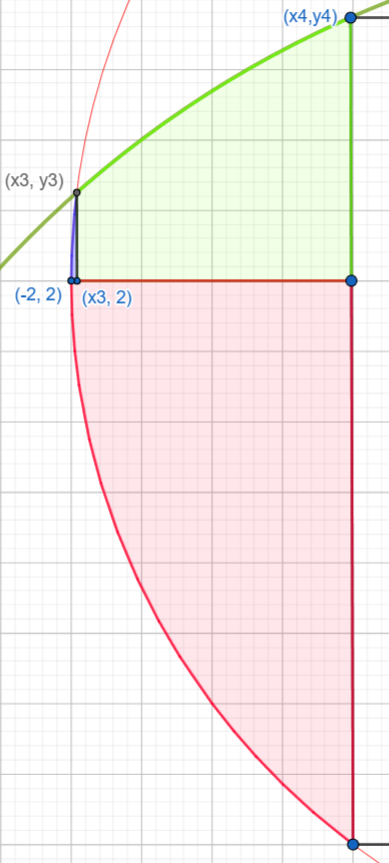
\includegraphics[width=5cm]{/images/problems/25_diagram4.png}
\end{center}
 
 Now we get the area of each part by integral: $$ \begin{aligned} A(\textsf{blue}) &= \int_{-2}^{x_3}\sqrt{4-x^2}dx \simeq 0.00262 \\ A(\textsf{green}) &= \int_{x_3}^{x_4}\sqrt{9-x^2}-2 dx \simeq 0.42644 \\ A(\textsf{red}) &= \int_{-2}^{x_4}2 - (-\sqrt{4-x^2} + 2) dx \simeq 0.92011 \end{aligned} $$ By adding the above three values, the answer to the problem is approximately 1.349.\end{solution}
